\documentclass[11pt,a4paper]{article}
\usepackage[UTF8,heading=true]{ctex}
\usepackage[a4paper,left=25mm,right=25mm,top=22mm,bottom=22mm]{geometry}
\usepackage{fontspec,xeCJK,graphicx,booktabs,tabularx,longtable,array,amsmath,amssymb,tikz}
\usetikzlibrary{arrows.meta,positioning}
\usepackage[hidelinks]{hyperref}
\setmainfont{Times New Roman}
\setCJKmainfont{SimSun}[BoldFont=SimHei]
\setCJKsansfont{SimHei}
\setlength{\parindent}{2em}
\setlength{\parskip}{3pt}
\linespread{1.18}
\setlength{\tabcolsep}{5pt}
\setlength{\abovecaptionskip}{5pt}
\emergencystretch=1.5em
\widowpenalty=10000
\clubpenalty=10000
\setcounter{secnumdepth}{3}
\ctexset{section={format=\Large\bfseries},subsection={format=\large\bfseries},subsubsection={format=\normalsize\bfseries}}
\graphicspath{{figures/}}
\makeatletter
\newenvironment{inlinefigure}{\par\addvspace{9pt}\noindent\begin{minipage}{\linewidth}\def\@captype{figure}\centering}{\end{minipage}\par\addvspace{9pt}}
\newenvironment{inlinetable}{\par\addvspace{7pt}\noindent\begin{minipage}{\linewidth}\def\@captype{table}\centering\small}{\end{minipage}\par\addvspace{7pt}}
\makeatother
\newcommand{\given}{\,|\,}
\pagestyle{plain}
% Generated only from saved research outputs; units defined in text.
\newcommand{\MainCost}{35126.85}
\newcommand{\MainPurchase}{59482.70}
\newcommand{\MainCharge}{20740.67}
\newcommand{\MainDischarge}{16799.94}
\newcommand{\MainLoss}{3940.73}
\newcommand{\PvCharge}{6247.96}
\newcommand{\RuleCost}{38276.64}
\newcommand{\ReserveCost}{37944.35}
\newcommand{\RulePurchase}{57742.42}
\newcommand{\ReservePurchase}{58060.96}
\newcommand{\RuleSaving}{3149.79}
\newcommand{\ReserveSaving}{2817.50}
\newcommand{\RuleSavingPct}{8.23}
\newcommand{\ReserveSavingPct}{7.43}
\newcommand{\ExtraPurchase}{1740.28}
\newcommand{\EveningState}{5168.13}
\newcommand{\PeakRulePurchase}{715.65}
\newcommand{\LowInitialCost}{35199.30}
\newcommand{\HighInitialCost}{35409.75}
\newcommand{\LowInitialDelta}{72.45}
\newcommand{\HighInitialDelta}{282.90}
\newcommand{\LowInitialPct}{0.21}
\newcommand{\HighInitialPct}{0.81}
\newcommand{\BuyTen}{0.00}
\newcommand{\BuyTwelve}{486.40}
\newcommand{\BuyFourteen}{0.00}
\newcommand{\BuySixteen}{394.93}
\newcommand{\BuyEighteen}{636.98}
\newcommand{\BuyTwenty}{0.00}
\newcommand{\ChargeA}{4500.00}
\newcommand{\DischargeA}{0.00}
\newcommand{\ChargeB}{833.33}
\newcommand{\DischargeB}{5947.42}
\newcommand{\ChargeC}{3954.63}
\newcommand{\DischargeC}{2121.42}
\newcommand{\ChargeD}{6119.37}
\newcommand{\DischargeD}{91.10}
\newcommand{\ChargeE}{0.00}
\newcommand{\DischargeE}{5068.69}
\newcommand{\ChargeF}{5333.33}
\newcommand{\DischargeF}{3571.31}

\begin{document}
\begin{center}\Large\bfseries 微网与外部电网电力调控策略\end{center}
\section{问题背景}
光伏发电能够为小区提供电力，但发电充足的时段与居民集中用电的时段未必一致。与外部电网相连的微网，可以从外网购电补充供给，也可以利用储能设备把电量留到以后使用。当光伏有剩余或外网电价较低时充电，在供电不足或电价较高时放电，是协调本地发电与用电需求的一种方式。

这种调控同时受到供电可靠性与购电成本的约束。提前多买电可能造成浪费，买得太少又可能在实际运行中产生高价补购；电池虽然能缓冲供需变化，却受到储电容量、充放电功率和能量损耗的限制。因此，微网需要根据决策时已经掌握的信息，协调各时段的购电与储能使用，在满足小区负载的前提下尽可能减少费用。

\section{问题重述}
\subsection{研究对象与共同条件}
研究对象为由光伏、储能设备和外网共同供电的小区微网。附件1给出代表日的电价、负载及光伏预测，附件2给出2025年全年的实际负载和光伏功率，附件3给出每天分四次发布的光伏预报，附件4给出同期波动电价。附件5提供各问的结果文件格式。

储能设备最大容量为12000 kWh，运行储电量须保持在1200--10800 kWh之间，最大充电和放电功率均为5000 kW。题目给定2025年1月1日零点储电量为6000 kWh。功率以kW表示，购电量、充放电量及储电量以kWh表示；各问均须保证微网供电满足小区负载。

\subsection{四问的具体任务}
\textbf{问题一：给定一天供需与电价时的购电安排。}根据附件1和储能参数，在零点安排当天的外网购电及储能充放电，要求当天零点与24点储电量相等。题目中的“每天相同”是指每日重复相同的电价和负载曲线，曲线在一天内仍可随时段变化。需给出满足供电要求、尽可能节省费用的具体安排。

\textbf{问题二：实际供需变化下的每日购电计划。}保持附件1的日内电价，利用附件2所对应的实际运行情景，在每天零点制定当天计划。普通购电按计划量计费；实际运行中供给不足的部分通过紧急购电补足，价格为相应电价的5倍。需同时给出每日计划、实际储能使用及紧急购电情况。

\textbf{问题三：利用更新预报调整购电计划。}在零点取得未来24小时整点光伏预报后制定当天计划，并可在6点、12点和18点取得新预报后调整尚未执行的购电安排。增加的购电量按相应电价的1.5倍收费，减少的部分涉及50\%的违约电价。需给出计划及调整结果，并判断引入日内预报是否值得。

\textbf{问题四：波动电价下的两类购电安排。}使用附件4的电价，分别重新研究问题二和问题三。两条分支分别保留原有的信息条件与调整权限，比较波动电价下的购电、储能使用和费用表现。

\subsection{结果范围与呈现要求}
完整购电结果按10分钟间隔提交。问题一至问题三分别填写\texttt{result1.xlsx}、\texttt{result2.xlsx}和\texttt{result3.xlsx}；问题四的两条分支分别填写\texttt{result4-2.xlsx}和\texttt{result4-3.xlsx}。问题二至问题四的完整结果覆盖2025年2月1日至12月31日，除计划购电和储能记录外，分别保留紧急购电及题目要求的调整记录。

论文按题目指定格式展示重点时段和日期，完整文件保留全部要求的记录。购电展示包括10、12、14、16、18和20点起始的六个10分钟区间，以及全天购电量和费用；储能展示按六个4小时区间分别汇总充电和放电，并列出日初与日末储电量。问题二、三重点展示3月20日、6月21日、9月23日和12月21日，并列出这些日期的紧急购电情况；问题四给出两条分支的相应结果。

\section{问题分析}
\subsection{问题一：电量在不同时段之间如何分配}
本问的主要矛盾是供需和电价在时间上的错配。某个时段光伏较多，并不意味着另一个时段无需购电；提前充电虽可减少后续高价购电，却会占用储能空间并产生损耗。因而，不能只比较一天的总发电量与总负载，也不能简单地在最低价时段尽量买满，而要同时考虑电量何时可得、何时需要，以及电池能否及时充入和放出。

日初与日末储电量相等，使当天的费用比较具有一致的起点和终点。若允许日末电量低于日初，就可能通过消耗初始库存减少当天购电，而把补回库存的费用留到以后。首尾相等消除了这部分表面节省，但并不要求电池全天保持同一电量；日内充放电仍是调控的主要手段。

\subsection{问题二：计划先制定，偏差后出现}
本问新增的困难是决策与实际信息出现的先后关系。附件2虽包含全年实际值，但每天零点尚未发生的负载和光伏不能直接用于当天计划。第二问没有另行提供当天供需预报，故需依靠此前已经发生的数据形成判断，并在运行时根据实际情况使用电池和紧急购电。

电池能够在实际光伏偏少或负载偏高时提供补充，也能吸收部分反向偏差，但其缓冲能力有限。即使当天总电量够用，缺电也可能先于富余电量出现；达到最低储电量或放电功率上限时，电池仍无法补足当前缺口。紧急购电的高价格使计划不能只追求普通购电量少，而应权衡预先多买的费用与不足时的补购风险。

连续运行还使每天的安排彼此关联：当天结束时留下多少电，会影响次日的应对能力。数据从1月1日开始，完整结果却从2月1日开始，二者之间的运行过程决定了2月初的可用储电量，不能直接把6000 kWh当作2月1日的初态。


\subsection{问题三：新信息的收益能否覆盖修改代价}
新预报使尚未执行的购电安排有机会更贴近实际需求，但修改订单本身有成本。部分预测变化可以由储能吸收，此时不一定需要改购电计划；若预计缺口超出储能可承担的范围，提前调增才可能比事后紧急购电更合算。调减同样需要比较退回购电款与违约费用。因此，预报更新是重新判断的依据，并不意味着每次都应修改订单。

本问还需要区分“获得预报的价值”与“日内继续更新预报的价值”。直接比较问题二与问题三，会同时包含零点新增光伏预报和日内更新的影响。评价日内预报时，应在具有相同零点信息的条件下，比较保留零点安排与利用后续预报调整的表现，才能说明6点、12点和18点的新信息究竟带来什么作用。

\subsection{问题四：供需变化之外还要面对价格未知}
按照本文采用的信息条件，未来真实电价在决策时不可提前获知。电价波动由此既影响购电费用，也影响提前充电是否值得、应保留多少电量以及何时使用储能。沿用原购电轨迹再更换价格，只能得到该轨迹的重新计价，不能回答价格变化后应怎样重新安排。

本问的两条分支必须分别研究。问题二对应的分支仍在零点制定普通购电计划；问题三对应的分支可在既定预报时刻调整未来安排。只有保留这一区别，才能分清价格不确定性和日内调整能力各自带来的影响，避免把额外的调整权限误当作某种购电方法的收益。

\section{总体思路}
四问围绕同一供电系统展开，共享负载满足、光伏利用、储电量变化及设备容量和功率限制。研究首先从问题一的一天安排入手，理清购电与储能转移电量之间的关系；再在问题二中加入实际供需偏差、紧急补购和跨日衔接，使当天计划与实际执行相区分。问题一形成的购电方案仅用于问题二首日启动，后续日期的计划则依据逐日积累的信息制定。

问题三在这一基础上引入按发布时间获得的光伏预报及有代价的计划调整，重点考察提前纠正偏差的作用。问题四分别扩展问题二和问题三，将固定日内电价替换为决策时尚未知晓的波动电价。这样，四问可以共用供电与储能的基本关系，同时分别处理供需偏差、信息更新和价格不确定性；费用比较也可明确对应到普通购电、调整和紧急购电三个来源。

\section{模型假设}
在题目给定的设备参数和交易规则基础上，作如下运行与信息假设，以明确电量流向、损耗计量及决策时可用的信息。

\textbf{（1）光伏优先直接供给小区负载。}光伏超过负载的部分可用于充电，外网购电既可直接供负载，也可给电池充电；三种电源允许共同供电。光伏优先是本文采用的运行约定。计划电量中能够即时使用或存储的部分予以接收，其余不接收，但普通购电仍按有效计划量结算。最终不能使用或储存的余电不计售电收入，也不对已支付的未利用电量重复计费。

\textbf{（2）采用固定充放电效率与外侧电量计量。}充电效率$\eta_{\mathrm c}$和放电效率$\eta_{\mathrm d}$均取0.90。充电量指进入储能设备前的电量，放电量指设备输出后可供负载使用的电量，5000 kW功率上限也按相应外侧计量。储电状态以电池内部电量表示，计算中不额外引入题目未给出的自放电和寿命折旧项。

\textbf{（3）以10分钟为调度区间。}问题一将附件1的每个采样值作为其后10分钟内的恒定功率和电价，以便将功率转换为时段电量。真实日期中的次日零点按实际日期衔接；问题一使用重复代表日，末尾零点标签映射到本周期开头。

\textbf{（4）储电状态连续衔接。}问题一主方案以6000 kWh开始，并在日末恢复到同一电量；不同起点的影响在本问灵敏度检验中单独考察。问题二至问题四承接前一天的剩余储电量，不逐日重置，也不将问题一的日首尾相等条件直接施加到后续每一天。

\textbf{（5）决策只使用当时可获得的信息。}问题二根据此前已经发生的负载、光伏及当前储电量制定计划，不使用附件3预报；问题三仅使用相应决策时刻已发布的预报。问题四未来实际价格不可提前获知，两条分支分别保留问题二和问题三的调整权限。问题二1月1日缺少更早历史，采用问题一基于附件1得到的购电结构启动，从6000 kWh连续运行，2月初电量由此前运行承接。

\textbf{（6）调整订单以零点原计划为统一结算基准。}对问题三及问题四的调整分支，最终有效普通订单减少部分退回原款，再收取该部分50\%的违约费用；增加部分按1.5倍价格计费，紧急购电另按5倍价格计费。多次修改时旧账冲回，重叠部分不重复收费，采用对应供电时段的价格。调整结果表记最终普通购电总量，零点计划和各次修改分别留存。

\section{符号说明}
以$d$表示日期，以$k$表示当天的10分钟区间。第$k$段为$[(k-1)\Delta t,k\Delta t)$，$k=1,\ldots,144$，$\Delta t=1/6$ h。$S_{d,0}$为当天零点储电量，$S_{d,k}$为第$k$段结束时的储电量，一天共对应145个状态边界。问题一只考虑一个代表日，以下模型中省略日期下标$d$。

功率、时段电量和库存分别表示供用电速率、该段累计电量及边界时刻的剩余电量。三者的主要符号与单位列于表\ref{tab:symbols}；决策量的电量流向在问题一模型中进一步说明。

{\small\renewcommand{\arraystretch}{1.18}
\begin{longtable}{>{\centering\arraybackslash}p{3.0cm}>{\raggedright\arraybackslash}p{8.2cm}>{\centering\arraybackslash}p{3.3cm}}
\caption{主要符号及其含义}\label{tab:symbols}\\
\toprule 符号 & 含义 & 单位或取值 \\ \midrule
\endfirsthead
\multicolumn{3}{c}{表\thetable\quad 主要符号及其含义（续）}\\
\toprule 符号 & 含义 & 单位或取值 \\ \midrule
\endhead
\bottomrule\endfoot
$d,\ k$ & 日期下标、日内时段索引 & $k=1,\ldots,144$\\
$\Delta t$ & 一个调度时段的长度 & $1/6$ h\\
$L_{d,k},\ P^{\mathrm{PV}}_{d,k}$ & 小区负载功率、光伏功率 & kW\\
$E^{\mathrm L}_{d,k},\ E^{\mathrm{PV}}_{d,k}$ & 负载电量、光伏电量；由相应功率乘$\Delta t$得到 & kWh\\
$p_{d,k}$ & 对应供电时段的电价 & 元/kWh\\
$m_{d,k}$ & 光伏直接供给负载的电量 & kWh\\
$n_{d,k},\ r_{d,k}$ & 光伏直供后的负载缺口、光伏富余电量 & kWh\\
$x_{d,k}$ & 外网购电中送入储能设备的电量 & kWh\\
$y_{d,k}$ & 送入储能设备的光伏电量 & kWh\\
$z_{d,k}$ & 储能设备输出给负载的电量 & kWh\\
$S_{d,k}$ & 第$k$段结束时的电池内部储电量 & kWh\\
$q_{d,k}$ & 外网购电总量；问题一中由电量分配关系确定 & kWh\\
$E^{\mathrm{ch}}_{d,k},\ E^{\mathrm{dis}}_{d,k}$ & 外侧总充电量$x_{d,k}+y_{d,k}$、总放电量$z_{d,k}$ & kWh\\
$w_{d,k}$ & 未被负载或电池利用的光伏电量 & kWh\\
$S_0$ & 问题一初始储电量，主方案取6000 & kWh\\
$S_{\mathrm{cap}}$ & 设备额定最大容量 & 12000 kWh\\
$S_{\min},\ S_{\max}$ & 允许运行的储电量下限、上限 & 1200、10800 kWh\\
$P_{\max}$ & 外侧充电或放电功率上限 & 5000 kW\\
$\eta_{\mathrm c},\ \eta_{\mathrm d}$ & 充电效率、放电效率 & 均为0.90\\
$C$ & 问题一全天普通购电费用 & 元\\
\end{longtable}}

\section{数据预处理与探索性分析}

\subsection{数据预处理}

本文使用题目附件中的代表日供需、全年实际负载与光伏、光伏预报及电价数据。预处理时，统一日期和时间的写法，将同一时刻的负载、光伏和电价对应起来，并保留每次发布的光伏预报。整理后的数值与原表逐项核对一致，没有改变原始数值。以下日均、月均功率按原表日期与采样标签分组取平均；原表末尾的次日零点仍随原标签参与这些描述统计。调度计算则按实际区间建立时间映射，问题一的周期零点单独对应到首段。

经过整理与分析，我们有以下发现。

\subsection{光伏富余与用电需求在时间上错开}

微网面临的首要问题是发电与用电在时间上的不一致。如图\ref{fig:reference}所示，光伏在白天逐渐增强，午间可以覆盖负载并产生富余；傍晚光伏回落后，小区仍有较高的用电需求。电价在晚间也处于较高水平，使这一阶段补充供电的成本更高。图中的负载与光伏功率差直观地反映了这种变化：午间出现富余，傍晚又需要外网或电池补充。

\begin{inlinefigure}
  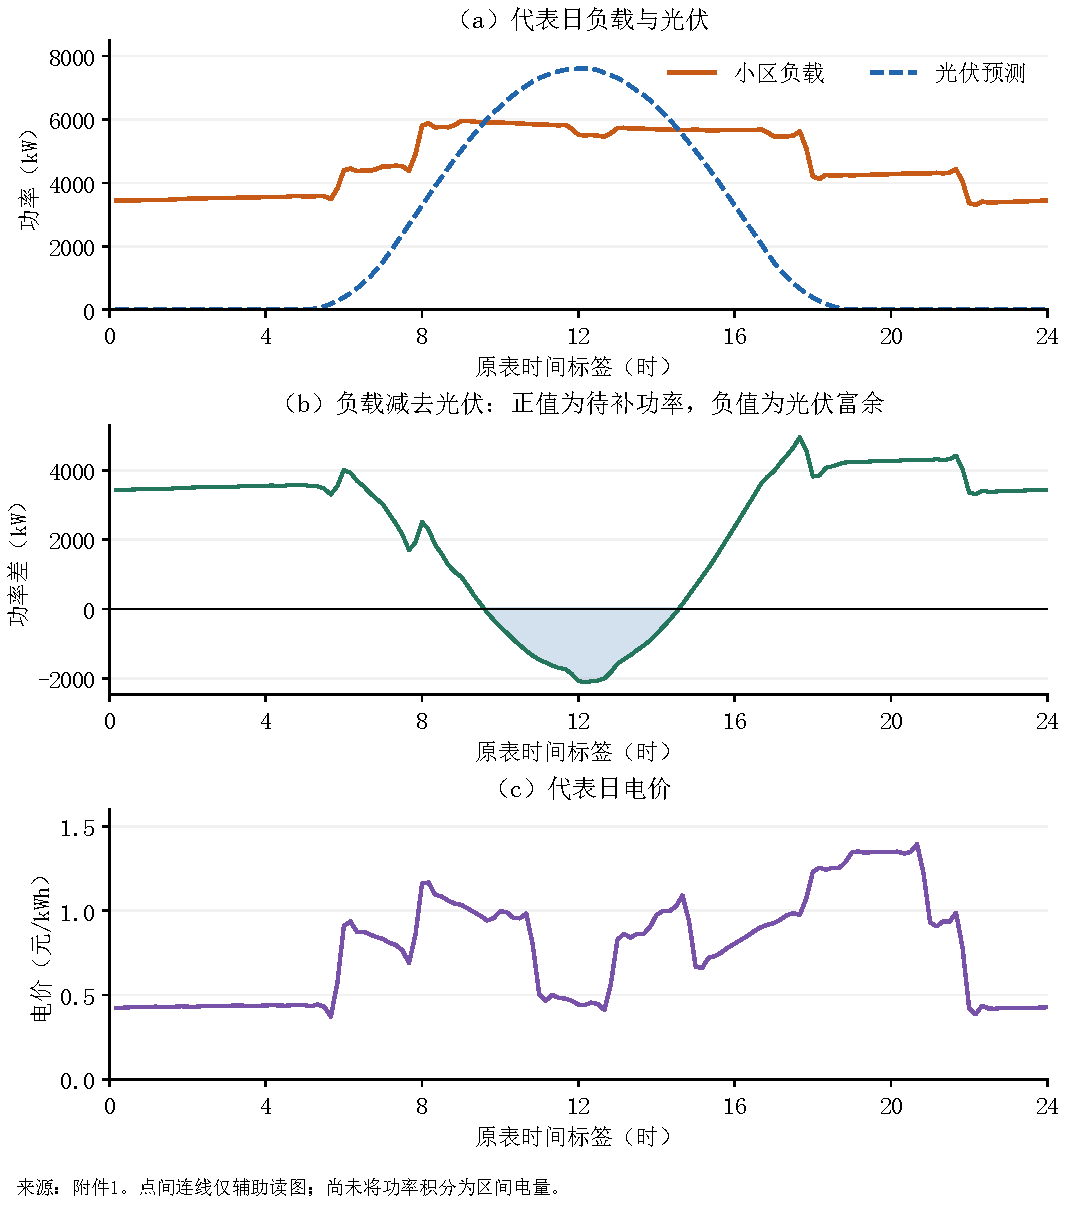
\includegraphics[width=0.82\linewidth]{01_reference_day.pdf}
  \caption{代表日供需与电价的时间错配}
  \label{fig:reference}
\end{inlinefigure}

代表日午间的最大富余功率约为2100 kW，而傍晚需要补充的功率最高接近5000 kW。这说明，白天发电充足并不能直接解决晚间供电问题。电池可以把部分富余电量留到以后使用，但必须先有空间接收，并能在需要时及时放出。因此，购电安排既与当时的供需差额有关，也与之前储存了多少电、之后还要应对多大需求有关。

这种时间错配并非仅出现在代表日：全年有330天出现过光伏超过负载的记录，接收和利用午间富余是经常需要面对的情景。不过，附件1接近全年各时刻的平均供需形状，具体日期仍会出现更高的负载峰值或不同程度的光伏富余。代表日能够说明储能转移电量的基本作用，却不足以代表每一天的运行压力。富余电量最终能利用多少，还取决于当时的电池状态，不能由富余出现的次数直接判断。

\subsection{用电高峰与供需缺口的季节变化不同步}

从图\ref{fig:annual}可以看到，负载与光伏都有明显的年内变化，但二者并不同步。夏季负载较高，同时也有较多光伏补充；进入冬季后，负载虽低于夏季高峰，光伏却明显减少。这使微网对外网补充的需求，不能仅按负载高低来判断。图中的逐日曲线还呈现出月均水平周围的持续起伏，说明季节变化与日际差异同时存在。

\begin{inlinefigure}
  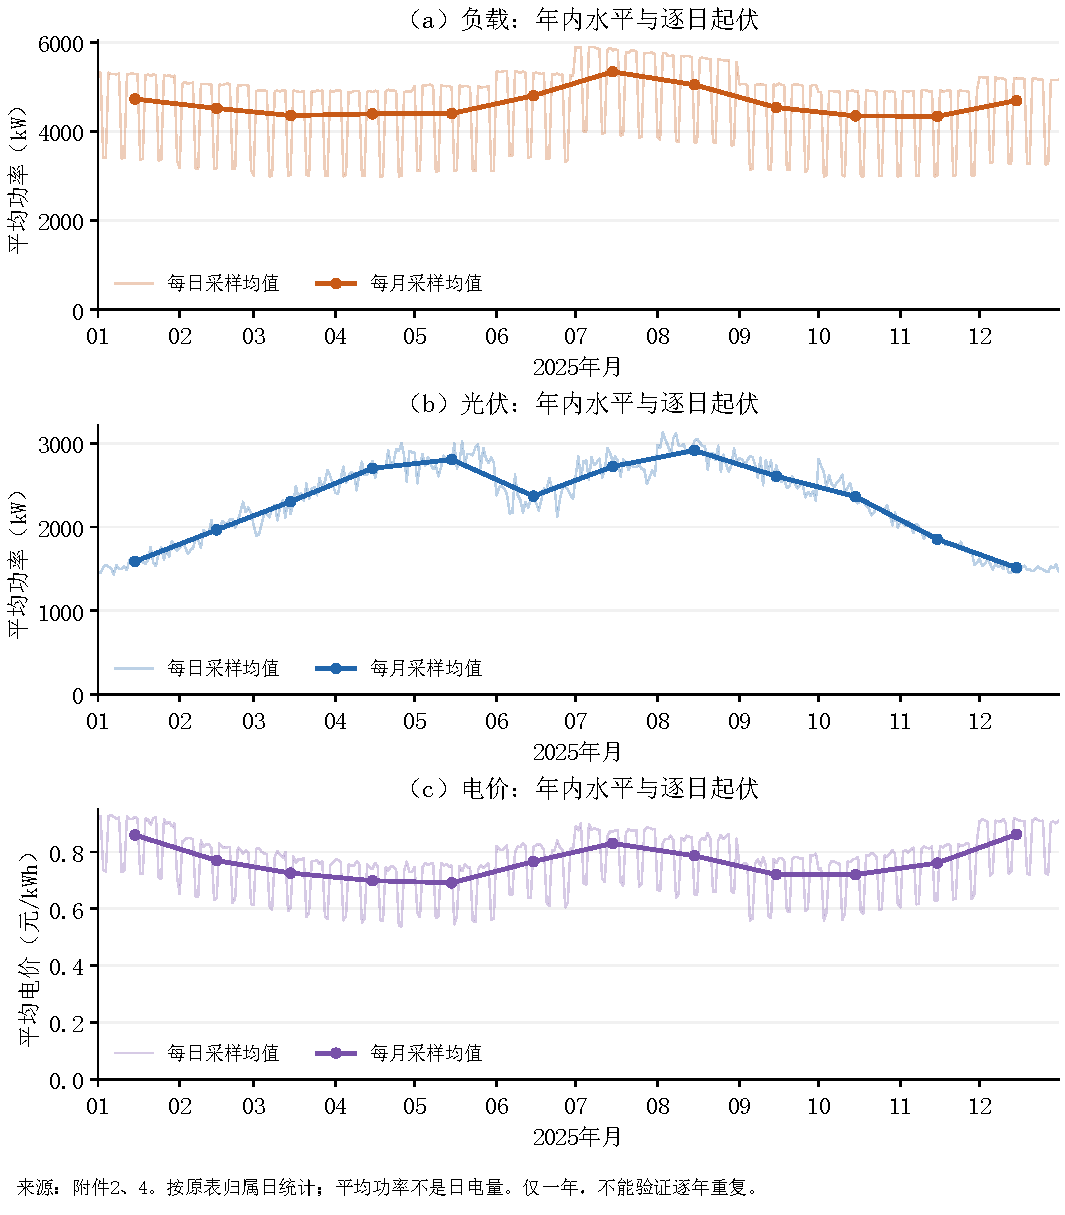
\includegraphics[width=0.82\linewidth]{02_year_and_month.pdf}
  \caption{负载、光伏与电价的年内变化}
  \label{fig:annual}
\end{inlinefigure}

以冬春差异为例，12月平均负载减去光伏后的功率差约为3180 kW，而5月约为1600 kW，前者接近后者的两倍。冬季供需差额较大，并不意味着用电一定更多，而是本地光伏能够承担的部分更少。对储能而言，这也意味着不同季节可供储存的光伏余量和随后需要补充的电力并不相同，全年照用同一套购电、充放电安排，难以适应这种变化。

年内变化也不是平滑的增减。例如，光伏月均功率在6月出现回落，低于相邻月份。附件没有对应天气资料，因此这里只将其视为实际数据中的变化，不推断具体气象原因。现有记录支持2025年存在明显季节差异，是否逐年以同样方式重复，还需要其他年份的数据验证。

\subsection{负载有周重复，电价仍存在跨日波动}

负载除了随季节变化，还表现出清楚的星期差异。按原始日期分组，周五和周六的平均负载比其余五天低约36.8\%，且各月均能观察到这一特点，见图\ref{fig:prices}。这意味着，相邻两天虽然在时间上更近，用电水平却未必更接近；参考历史负载时，同一星期位置的记录也可能提供有用信息。该分组来自附件日期，不据此推断居民的具体作息制度。

\begin{inlinefigure}
  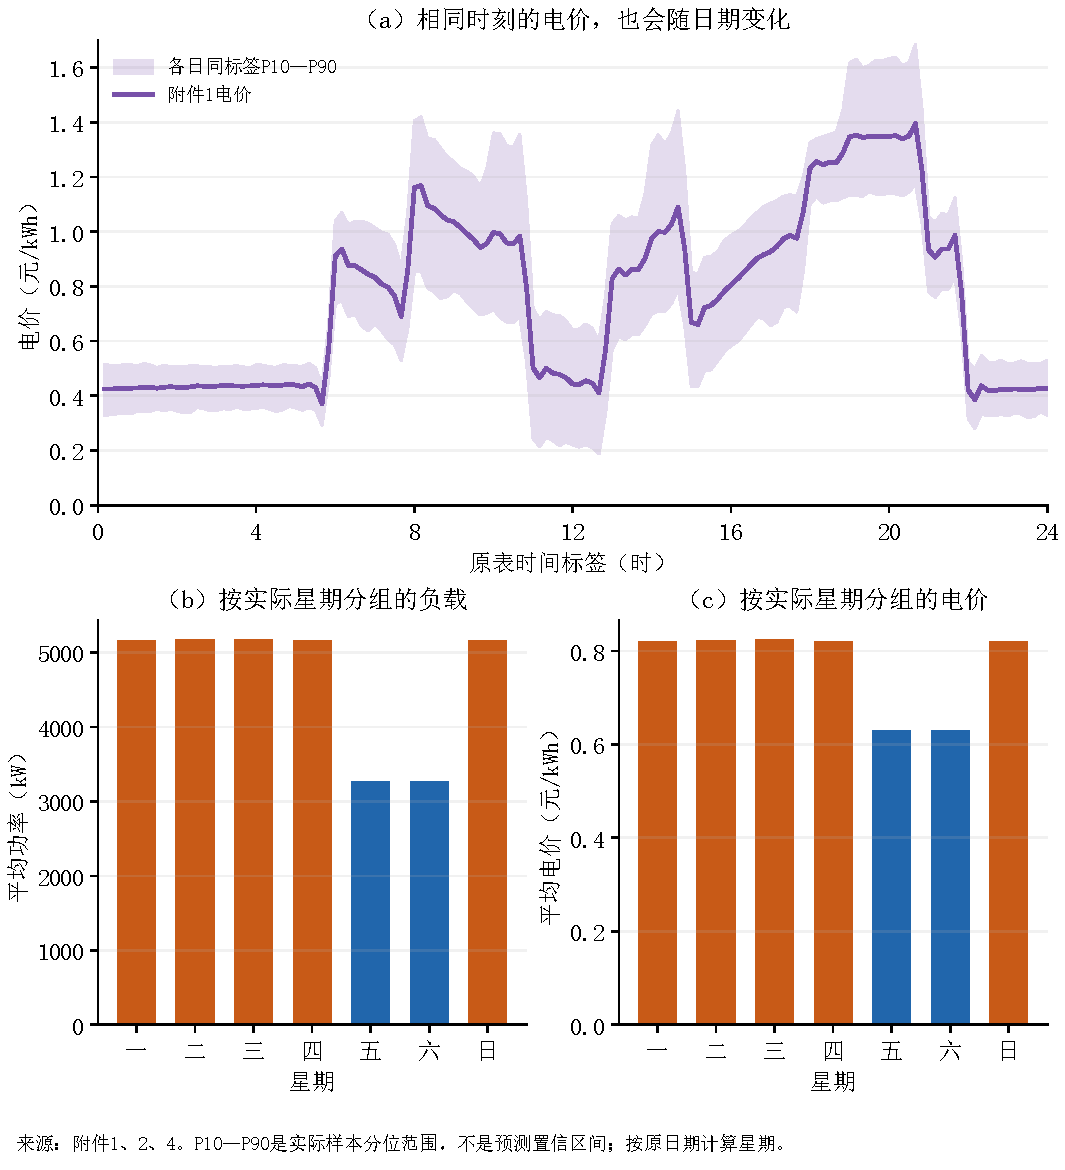
\includegraphics[width=0.78\linewidth]{06_prices_and_weekdays.pdf}
  \caption{不同星期的用电差异与同一时刻的电价波动}
  \label{fig:prices}
\end{inlinefigure}

将序列与一周前的数值比较，并扣除各月相同时刻的平均轮廓后，负载和电价仍保持较强的相关性，而光伏的一周相关性已接近零。光伏原先较高的相似程度，主要来自白天发电、夜间接近零的共同形状。因此，这几类数据不能仅因都呈现重复起伏，就被视为具有相同的周规律；历史信息的参考方式需要适应各自的变化特点。

电价还存在同一时刻、不同日期之间的差异。图\ref{fig:prices}中的阴影给出全年各日同一时刻价格的第10至第90百分位范围，其宽度反映出固定日内曲线没有呈现的波动。历史上较便宜的时段仍可作为参考，但并不保证下一天也同样便宜。按第四问采用的信息条件，未来真实价格尚不可知，提前充电的收益也就存在不确定性：低价购电能否弥补充放电损耗，取决于之后实际遇到的价格和用电需求。

\subsection{光伏预报更新的改善与局限}

附件3的预报整体呈现出提前越久、误差越大的特点，如图\ref{fig:forecast}所示。比较时，将预报与同一目标整点的实测值对应，以两者绝对差的平均值衡量偏差；年末超出实测覆盖范围的36条预报不参与误差计算。图中还区分了全部记录与实际有光伏的记录：夜间接近零的数值会降低总体平均误差，因此仅看总体结果，容易忽略实际发电时更大的供需偏差。

\begin{inlinefigure}
  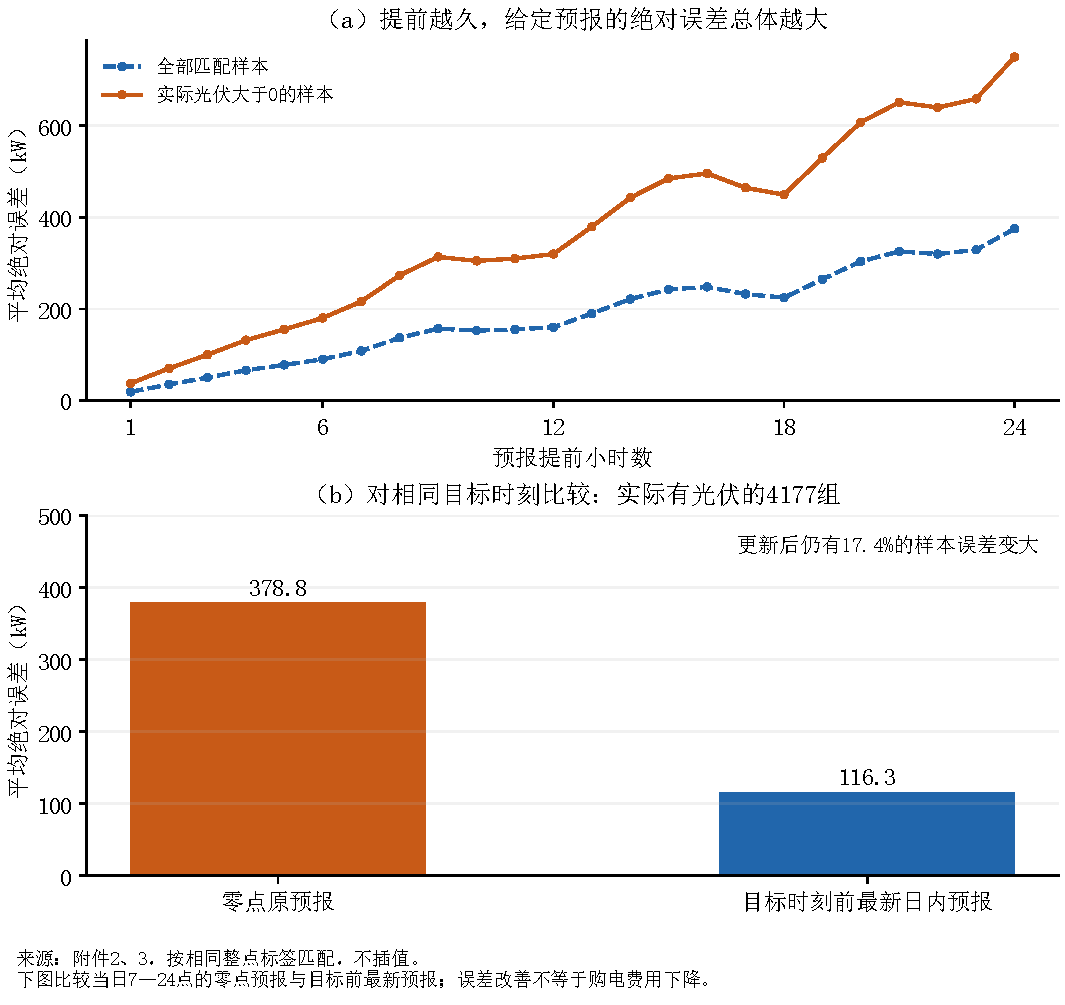
\includegraphics[width=0.78\linewidth]{07_forecast_accuracy.pdf}
  \caption{预报提前量与日内更新对光伏预报误差的影响}
  \label{fig:forecast}
\end{inlinefigure}

为直接观察更新的作用，对每天7点至24点的同一目标时刻，比较零点预报与目标发生前已经发布的最新预报。在实测光伏大于零的4177组配对中，平均绝对误差由约379 kW降至116 kW，减少约69\%。这说明，日内更新确实改善了这组数据中对未来光伏的判断。不过，仍有约17.4\%的配对在更新后误差增大，新预报并非每次都更准确。这里按实测值分组是为了观察发电时的误差，制定计划时并不能提前知道实际光伏。

更准确的信息为调整购电提供了依据，但其经济作用还取决于电池和合同。如果原计划的偏差可以由电池吸收，修改购电量未必划算；如果预计偏差较大、储能又缺少调节余地，提前调整才可能减少昂贵的紧急补购。预报更新的价值取决于它是否改变了实际需要的购电量，以及节省的补购费用能否抵偿调整费用，不能直接用平均误差的降幅代表节费比例。

\section{模型的建立与求解}
\subsection{问题一的建立与求解}

附件1给出了同一天内的供需和电价曲线，问题一的关键在于把有限的储能用在合适的时段。若仅在电价低时充电、电价高时放电，可能过早占满午间所需的储能空间，也可能在真正的价格高峰到来前用完可放电量。因此，本文以各时段的电量分配为决策对象，将全天购电和储能变化联系起来，并与两种直观的峰谷购电策略比较，以确定问题一采用的方案。

\subsubsection{时段划分与决策变量}
将一天分为144个10分钟区间，使用第$k$段起点的采样值代表该段内的功率。相应的负载电量与光伏电量为
\begin{equation}
 E^{\mathrm L}_k=L_k\Delta t,\qquad E^{\mathrm{PV}}_k=P^{\mathrm{PV}}_k\Delta t,
 \qquad \Delta t=\frac{1}{6}\ \mathrm h.
 \label{eq:energy_conversion}
\end{equation}
例如，某段负载功率为6000 kW，该10分钟所需电量为1000 kWh。输入表中的零点虽排在末尾，但在重复代表日内对应第一段00:00--00:10；其余记录按实际时刻对应区间，而不直接以行号表示时间。

按光伏优先直接供负载的假设，先计算直供电量$m_k$、剩余负载缺口$n_k$和光伏富余$r_k$：
\begin{equation}
 \begin{aligned}
 m_k&=\min\{E^{\mathrm L}_k,E^{\mathrm{PV}}_k\},\\
 n_k&=E^{\mathrm L}_k-m_k,\qquad r_k=E^{\mathrm{PV}}_k-m_k.
 \end{aligned}
 \label{eq:pv_first}
\end{equation}
这三项均由已知数据确定。它们将同一时段分为负载需要补电或光伏存在富余两种情形，避免将本可直接使用的光伏先送入电池而产生不必要的损耗。

每段设置四个连续决策量：外网用于充电的电量$x_k$、光伏用于充电的电量$y_k$、电池向负载输出的电量$z_k$，以及段末内部储电量$S_k$。四者均以kWh计量，但前三者按设备外侧计量，$S_k$按电池内部计量。为说明购电量与这些变量的关系，将电量流向整理为图\ref{fig:energy_paths}。

\begin{inlinefigure}
 % Q1 energy-path definition: report 12.2, 15; external-side kWh.
\begin{tikzpicture}[>=Stealth, node distance=16mm, every node/.style={font=\small},
  box/.style={draw=black,rounded corners=2pt,minimum width=23mm,minimum height=10mm,align=center},
  lab/.style={fill=white,inner sep=2pt}]
\node[box] (grid) at (0,1.25) {外部电网};
\node[box] (pv) at (0,-1.25) {光伏发电};
\node[box] (battery) at (5,0) {储能设备\\$S_{k-1}\longrightarrow S_k$};
\node[box] (load) at (10,1.25) {小区负载};
\node[box] (waste) at (10,-1.25) {未利用光伏};
\draw[->] (grid.east) -- node[lab,above] {$n_k-z_k$} (load.west);
\draw[->] (grid.south east) -- node[lab,above,sloped] {$x_k$} (battery.north west);
\draw[->] (pv.north east) -- node[lab,above,sloped] {$y_k$} (battery.south west);
\draw[->] (battery.north east) -- node[lab,below,sloped] {$z_k$} (load.south west);
\draw[->] (pv.south) -- (0,-2.65) -- node[lab,below] {$m_k$：光伏直供} (11.9,-2.65) -- (11.9,1.25) -- (load.east);
\draw[->] (pv.east) -- node[lab,pos=.70,above] {$w_k=r_k-y_k$} (waste.west);
\end{tikzpicture}

 \caption{问题一的电量分配关系（各箭头表示该时段的电量）}
 \label{fig:energy_paths}
\end{inlinefigure}

图中，外网既补足电池放电后的负载缺口，也可为以后使用而充电，因此总购电量为
\begin{equation}
 q_k=n_k-z_k+x_k. \label{eq:purchase}
\end{equation}
总充电量为$E^{\mathrm{ch}}_k=x_k+y_k$，总放电量为$E^{\mathrm{dis}}_k=z_k$；未利用光伏为$w_k=r_k-y_k$。这样，购电量不再需要作为独立变量，供电和储能的每一条去向仍可单独核对。

\subsubsection{目标函数}
问题一只计普通外网购电费用。光伏为小区提供本地电源，储能损耗通过额外所需的购电量反映，不另加一笔损耗费用；题目也未给出售电收入或电池寿命成本。因此，以全天购电费用最小为目标：
\begin{equation}
 \min C=\sum_{k=1}^{144}p_kq_k
       =\sum_{k=1}^{144}p_k(n_k-z_k+x_k).
 \label{eq:objective}
\end{equation}
这里$p_k$的单位是元/kWh，$q_k$已经是10分钟电量，计算费用时不再乘$\Delta t$。目标最小化的是费用，而非购电总量；适度增加低价购电，即使带来充放电损耗，也可能减少更昂贵时段的购电支出。

\subsubsection{约束条件}
\textbf{（1）供电与光伏分配。}各时段的负载均需得到满足，充入电池的光伏不能超过该段富余，电池放电不能超过直供后的缺口：
\begin{equation}
 \begin{gathered}
 x_k\geq0,\qquad 0\leq y_k\leq r_k,\qquad 0\leq z_k\leq n_k,\\
 m_k+(q_k-x_k)+z_k=E^{\mathrm L}_k,\qquad
 m_k+y_k+w_k=E^{\mathrm{PV}}_k,\quad w_k\geq0.
 \end{gathered}
 \label{eq:balance}
\end{equation}
其中两条等式由式\eqref{eq:pv_first}和式\eqref{eq:purchase}直接保证。$q_k-x_k=n_k-z_k$为外网直接供负载的电量；允许富余光伏无法全部存入，但不给未利用电量附加售电收益。

\textbf{（2）充放电功率。}容量表示能存多少，功率表示每段能充入或放出多快。最大充电功率和放电功率均为5000 kW，故
\begin{equation}
 x_k+y_k\leq P_{\max}\Delta t,\qquad z_k\leq P_{\max}\Delta t,
 \qquad P_{\max}=5000\ \mathrm{kW}.
 \label{eq:power}
\end{equation}
每段外侧充电量或放电量因此不超过833.33 kWh。此上限约束储能设备，外网直接向负载供电的部分不占用电池充放电功率。

\textbf{（3）储电量变化及运行区间。}充电损耗发生在电量进入电池时，放电损耗发生在电量输出时，故
\begin{equation}
 S_k=S_{k-1}+\eta_{\mathrm c}(x_k+y_k)-\frac{z_k}{\eta_{\mathrm d}},
 \qquad \eta_{\mathrm c}=\eta_{\mathrm d}=0.90,
 \label{eq:soc}
\end{equation}
\begin{equation}
 1200\leq S_k\leq10800,\qquad k=1,\ldots,144.
 \label{eq:soc_bound}
\end{equation}
向设备输入100 kWh只能使内部库存增加90 kWh，而向负载输出90 kWh需要从内部扣除100 kWh。因此，外部电量经过一次完整充放后，能够用于负载的比例为$0.9\times0.9=0.81$。设备达到1200 kWh下限即不能继续放电，并不需要等到电量降至零。

\textbf{（4）日首尾电量相等。}主方案取日初储电量6000 kWh，并要求
\begin{equation}
 S_0=S_{144}=6000\ \mathrm{kWh}.
 \label{eq:cyclic}
\end{equation}
将式\eqref{eq:soc}对全天求和可得
\begin{equation}
 \sum_{k=1}^{144}z_k=\eta_{\mathrm c}\eta_{\mathrm d}
 \sum_{k=1}^{144}(x_k+y_k)=0.81\sum_{k=1}^{144}(x_k+y_k).
 \label{eq:daily_energy}
\end{equation}
这说明当天输出的储能电量需要由当天充电补回，不能依靠消耗初始库存制造低费用。6000 kWh确定主方案的比较条件，日内储电量仍可在允许区间内变化。

\subsubsection{线性结构与求解方法}
上述目标与约束均为线性关系。式\eqref{eq:pv_first}虽然含有最小值运算，但作用于已知供需数据，并未引入非线性决策。每段四个变量，共576个连续变量，144条储电递推等式将全天安排联系起来。

还需说明为何没有额外设置充电、放电的二元开关。在本问正电价、外网可直接供负载的条件下，同时充放电只会增加损耗。若某段$x_k>0$且$z_k>0$，则$n_k>0$、$r_k=0$，因而$y_k=0$。令$\delta=\min\{x_k,z_k/0.81\}>0$，将$x_k$减少$\delta$，同时将$z_k$减少$0.81\delta$，则
\begin{equation}
 \Delta S_k=-0.9\delta+\frac{0.81\delta}{0.9}=0,
 \qquad \Delta q_k=-0.19\delta<0.
 \label{eq:no_cycle}
\end{equation}
这一调整不改变储电轨迹，不破坏功率或供电约束，却严格降低费用，故同时充放不可能是最优选择。因此，本问可直接采用连续线性规划；若出现负电价或新增离散开关限制，这一结论需重新检验。

求解时，先按时间映射生成144段电量与价格，再将式\eqref{eq:objective}和式\eqref{eq:balance}--\eqref{eq:cyclic}整理成线性规划的系数矩阵与变量上下界，使用SciPy的\texttt{linprog}接口调用HiGHS。求解器以最优状态正常终止，并输出逐段购电、充放电与储电量。数值最优性及逐段约束另作独立复核，结果见本问检验部分。

\subsubsection{模型比较与方案选择}
为判断全天统一安排的实际收益，设置两种具有直观含义的参照策略。峰谷电价策略根据低价、高价门槛及目标储电量安排充放电，并考虑充放电损耗；光伏空间预留策略在相同规则上，进一步根据后续富余光伏限制提前充电，避免过早占满电池。线性规划则不预设价格门槛，而是在同一供需与设备条件下，同时确定所有时段的安排。

比较统一使用附件1的代表日、充放各90\%的效率及首尾6000 kWh条件。两种规则分别考察27组相同的参数组合：低价门槛取电价的15\%、25\%、35\%分位，高价门槛取65\%、75\%、85\%分位，目标储电量取6000、8400、10800 kWh。两者均按剩余时段的充放能力保护日末目标，恢复库存所需的实际购电全部计费，再分别取所考察组合中费用最低的结果。

峰谷电价策略、光伏空间预留策略与线性规划的全天费用依次为\RuleCost{}元、\ReserveCost{}元和\MainCost{}元。线性规划相较前两者分别节省\RuleSaving{}元和\ReserveSaving{}元，降幅为\RuleSavingPct{}\%和\ReserveSavingPct{}\%，且三种入选安排均满足逐段约束、没有未利用光伏。由此，本文选择线性规划作为问题一的购电与储能调度方案。它的优势既有实际费用比较的支持，也有在所列约束下统筹全天电量的结构依据。

光伏预留本身的作用并非在所有参数下都相同。在27组相同参数的配对中，18组费用降低、9组相同；尤其在峰谷策略费用最低的那组参数下，加入光伏预留并未改变结果。因此，预留策略各自调参后的费用较低，不能全部归因于新增预留机制。上述比较限于给定代表日和已考察的规则参数，不将规则的局部搜索结果称为该类方法的全局最优，也不据此评价未实际运行的其他算法。

\subsubsection{购电安排与结果分析}
主方案全天购电\MainPurchase{} kWh，费用\MainCost{}元，储能外侧累计充电\MainCharge{} kWh、累计放电\MainDischarge{} kWh。题目指定的六个购电区间及4小时储能汇总分别列于表\ref{tab:purchase}和表\ref{tab:storage}，其余10分钟购电结果保存在\texttt{result1.xlsx}中。

\begin{inlinetable}
 \caption{问题一指定区间的购电量及全天费用}\label{tab:purchase}
 \renewcommand{\arraystretch}{1.23}
 \begin{tabularx}{\linewidth}{l*{3}{>{\centering\arraybackslash}X}}
 \toprule
 时间段 & 10:00--10:10 & 12:00--12:10 & 14:00--14:10\\
 购电量/kWh & \BuyTen & \BuyTwelve & \BuyFourteen\\ \midrule
 时间段 & 16:00--16:10 & 18:00--18:10 & 20:00--20:10\\
 购电量/kWh & \BuySixteen & \BuyEighteen & \BuyTwenty\\ \midrule
 全天购电量/kWh & \multicolumn{3}{c}{\MainPurchase}\\
 全天购电费/元 & \multicolumn{3}{c}{\MainCost}\\
 \bottomrule
 \end{tabularx}
\end{inlinetable}

\begin{inlinetable}
 \caption{问题一各4小时区间的储能充放电量}\label{tab:storage}
 \renewcommand{\arraystretch}{1.23}
 \begin{tabularx}{\linewidth}{l*{3}{>{\centering\arraybackslash}X}}
 \toprule
 时间段 & 00:00--04:00 & 04:00--08:00 & 08:00--12:00\\
 充电量/kWh & \ChargeA & \ChargeB & \ChargeC\\
 放电量/kWh & \DischargeA & \DischargeB & \DischargeC\\ \midrule
 时间段 & 12:00--16:00 & 16:00--20:00 & 20:00--24:00\\
 充电量/kWh & \ChargeD & \ChargeE & \ChargeF\\
 放电量/kWh & \DischargeD & \DischargeE & \DischargeF\\ \midrule
 零点储电量/kWh & \multicolumn{3}{c}{6000.00}\\
 24点储电量/kWh & \multicolumn{3}{c}{6000.00}\\
 \bottomrule
 \end{tabularx}
\end{inlinetable}

4小时内同时出现充电量和放电量，表示这些动作发生在其中不同的10分钟区间；逐段结果没有同时充放电。全天累计充电量超过设备容量也不矛盾，因为电池在一天内可以反复使用，容量限制的是某一时刻的库存。

线性规划在凌晨补充电量，在早间用电阶段释放一部分库存，并利用午间富余光伏和适当的外网充电为晚间作准备。到16点，电池储电量达到10800 kWh。晚间虽已进入较高电价区间，方案仍保留一部分电量等待更贵的时段：20点尚有\EveningState{} kWh，而两种规则策略均已降至1200 kWh下限。20:40--20:50电价达到1.3952元/kWh时，线性规划由电池补足负载缺口，该段外网购电为零；两种规则则仍需购买\PeakRulePurchase{} kWh。日末价格回落后，方案再补回6000 kWh的起始库存。

节费并非来自减少所有购电。相较峰谷规则，线性规划多购电\ExtraPurchase{} kWh，恰好对应更多充放电带来的额外损耗；三种入选策略均已利用全部富余光伏，光伏利用率也不是这里费用差异的来源。真正的收益在于以更多低价电替代高价电。以外网充电为例，在低价$p_a$时购买1 kWh，经充放后只能替代高价$p_b$时的0.81 kWh，只有$p_a<0.81p_b$才具有基本价格收益；实际能转移多少，还受容量、功率和后续供需共同限制。

上述购电与储能变化可结合图\ref{fig:dispatch}理解。图中将三种策略的电价、储电量和购电功率放在同一时间轴上。上图帮助定位高价时段，中图说明电量何时留存、何时使用，下图给出相应的外网购电变化。

\begin{inlinefigure}
 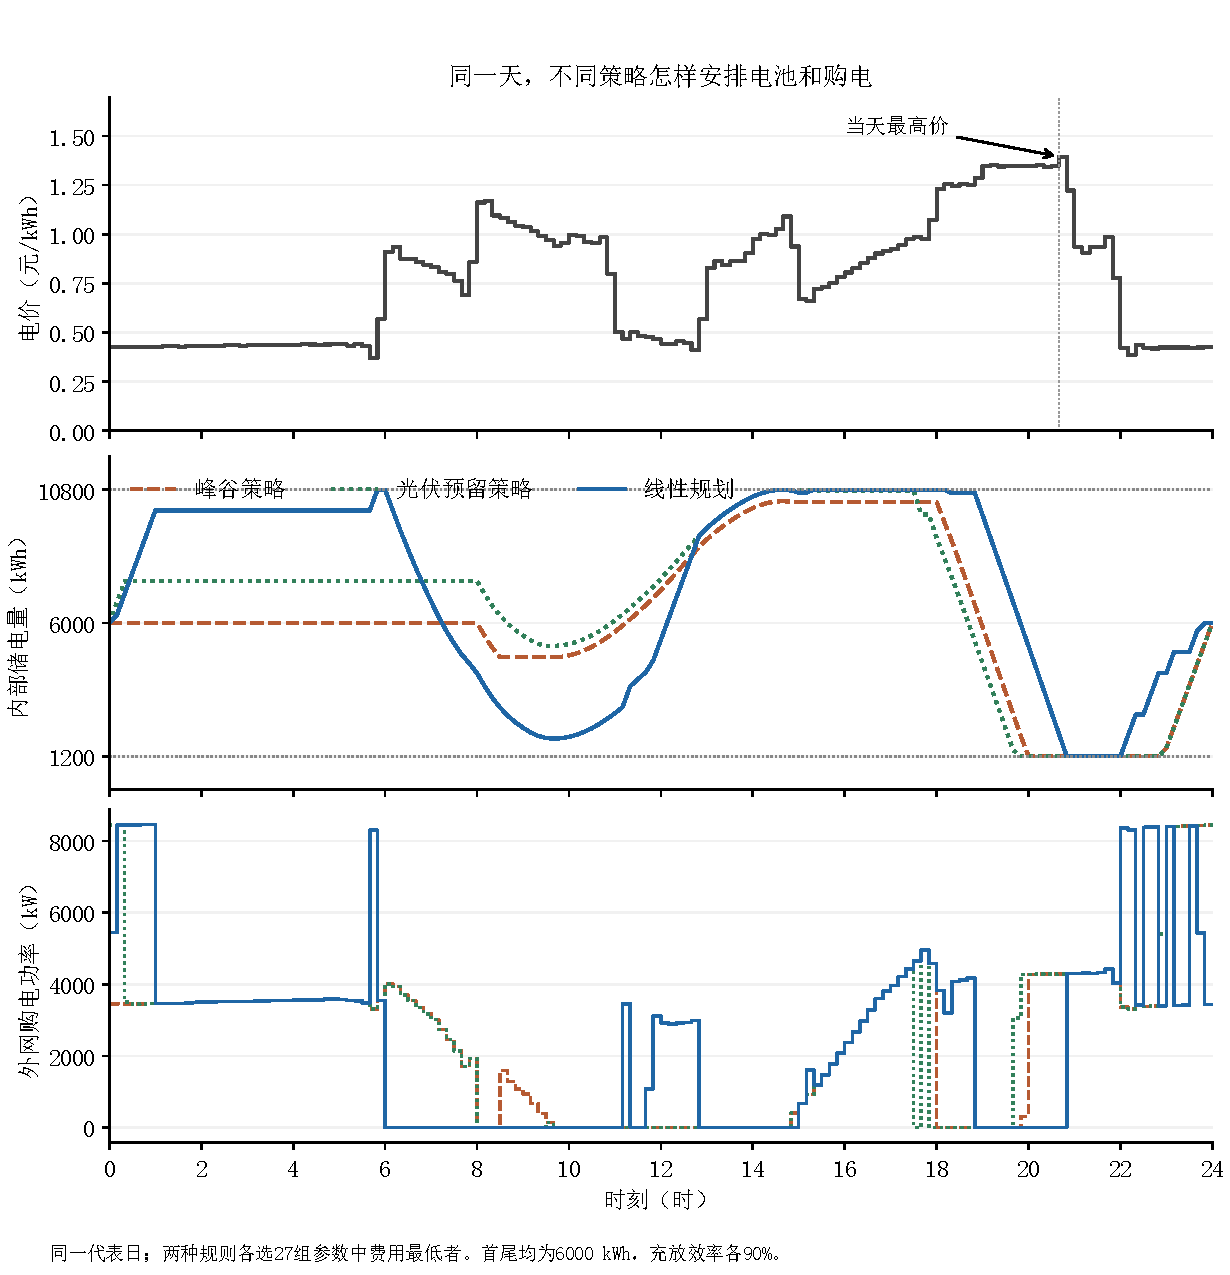
\includegraphics[width=0.90\linewidth]{q1_daily_dispatch.pdf}
 \caption{三种策略在相同代表日下的购电与储能安排}
 \label{fig:dispatch}
\end{inlinefigure}

\subsubsection{模型检验与初始储电量敏感性分析}
首先按导出的10分钟结果独立复算供需平衡、储电递推、容量与功率上限及全天费用，并核对首尾电量。三个起点案例的最大储电递推残差约为$1.34\times10^{-12}$ kWh；由求解器对偶信息独立重算的费用下界与实际可行方案费用之差最大约为$1.22\times10^{-12}$元。可行费用与下界在数值精度内一致，支持所列线性规划的最优性判断。此外，通过同价充放无套利、低高价两段充放以及初始库存不能免费消耗的小例子核对损耗与边界表达，并将导出表按真实时间逐项对应，避免零点置末造成结果错位。

问题一要求首尾电量相同，但相同的起点数值仍可能影响当天安排。为考察这种影响，保持供需、电价、效率和设备条件不变，分别以1200、6000和10800 kWh开始，每种情况均重新优化，并在日末恢复到各自起点。所得费用分别为\LowInitialCost{}元、\MainCost{}元和\HighInitialCost{}元；相较6000 kWh主方案，两个边界起点分别增加\LowInitialDelta{}元和\HighInitialDelta{}元，增幅为\LowInitialPct{}\%和\HighInitialPct{}\%。

三个案例的全天购电、累计充放电和光伏利用量相同，20点也都保留约\EveningState{} kWh，并避开最高价区间购电。但费用接近不表示逐段安排不变：两个替代起点各有14段购电量改变，均将5333.33 kWh从一部分时段转移到另一部分时段。低起点少了4800 kWh内部库存，凌晨需要多买$4800/0.9=5333.33$ kWh补充，日末则相应少补；高起点虽能减少凌晨补电，却必须在日末恢复更多库存。受充电功率和剩余时间限制，高起点还需在21:50--22:00以0.7764元/kWh额外购买666.67 kWh，因而开始时电量更多并不保证全天费用更低。

这三个已检验起点下，重新安排后的费用差异均不到1\%，且为晚间高价时段留电的特征保持一致；初始电量主要改变凌晨与日末的补电分配。检验只覆盖这三个取值，不能据此认定6000 kWh是整个允许区间内的最佳起点，也不能将重新优化后的结果解释为固定计划能够抵抗供需预测误差。问题一给出的是已知代表日下的调度依据；实际供需偏差出现后，计划与执行之间的差异还需在后续问题中处理。

\end{document}
